\section{Analysing aSTEP-2019} \label{sc:astep2019}
In this section, we analyze the different parts of \gls{astep}-2019.

\subsection{User Interface}
\gls{astep}-2019 divide programs into services. Services can be accessed directly through the \gls{ui}, or a service can provide an \gls{api} to other services. To be accessed through the \gls{ui}, a service must expose specific resources at predetermined \glspl{endpoint}. These \glspl{endpoint}, as well as a brief description of their purpose, can be seen in Table \ref{tab:endpoints}.

\bgroup
\def\arraystretch{1.8}
\begin{table}[htbp]
    \centering
    \begin{tabular}{|c|M{100mm}|}
        \hline
        Endpoint & Purpose \\ 
        \hline
        /info    & Exposes info about a service, such as name, category and version of \gls{ui} to use, for the \gls{ui} to display. \\ 
        \hline
        /fields  & Exposes information about which user input fields to render in the \gls{ui} sidebar. \\ 
        \hline
        /readme  & Documentation for a service. The will be displayed when service is accessed. \\ 
        \hline
        /render  & Provides information about how to render a service, both before and after information has been submitted in the fields. \\ 
        \hline
    \end{tabular}
    \caption{\Glspl{endpoint} that must be exposed by a service, for it to be rendered in the \gls{ui}.}
    \label{tab:endpoints}
\end{table}
\egroup

\noindent
All of these \glspl{endpoint} must allow for the \gls{http} method GET, except for /render, which must provide both GET and POST. /render must be accessible, even without submitted data. When a service exposes these \glspl{endpoint}, it will show up in the sidebar and become accessible. The \gls{ui} is consistent and stable, so there is no need to change it.

\subsection{Documentation} \label{sc:documentation}
\gls{astep}-2019 splits documentation between several different locations. A \gls{rfc} list contains the most up-to-date versions of documentation for most of \gls{astep}. The \gls{rfc}-list structures documentation as a proposal for a change to the system. Furthermore, ReadMe files on individual GitLab repositories sometimes contain documentation. Finally, documentation for specific services can be found in the service \gls{ui} and will be displayed as the first thing when accessing the service. This means that to find specific documentation for \gls{astep}-2019, at least three different locations must be searched. We propose that this system be changed.

\subsection{Analytics Platform}
There is currently no shared analytics platform. Each service individually implements analytics, with no means to share analytics between services. Having a shared platform, could remove redundant code and provide a more decoupled system in line with the microservices architecture currently implemented. We imagine the possibility of improvement to this area.

Furthermore, there is no microservice for anomaly detection. Which means that we must construct our anomaly detection service from the ground up.

\subsection{Server Architecture}
The server architecture for \gls{astep}-2019 uses a \gls{kubernetes} cluster as the primary server, hosting the different services. It has separate servers for hosting GitLab, building services into \gls{docker} images, and for running the \gls{ui}. \gls{cicd} is implemented through GitLab in tandem with the build server. The \gls{cicd} can automatically build GitLab repositories into a \gls{docker} image and deploy it to the \gls{kubernetes} cluster. Figure \ref{fig:server_architecture}. shows a sketch of the server architecture. 

\begin{figure}
    \centering
    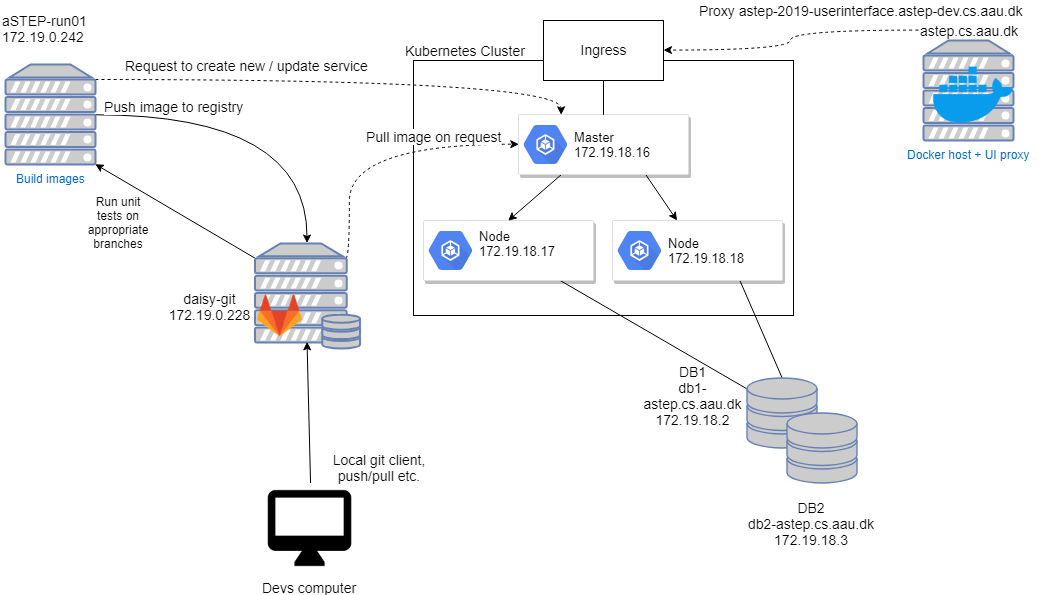
\includegraphics[width=0.9\textwidth]{Pictures/Sprint_1/server_architecture.png}
    \caption{A sketch of the server architecture of \gls{astep} \cite{astep}}
    \label{fig:server_architecture}
\end{figure}

The server architecture for \gls{astep}-2019 is robust and do not need to be changed.

\subsection{Database}
There are two different \gls{postgres} database servers (depicted as db1 and db2 in Figure \ref{fig:server_architecture}) connected to the \gls{astep} project. The databases can be used either directly with SQL queries or indirectly using a micro-service such as a \gls{graphql} service. The \gls{kubernetes} micro-service architecture has allowed each group to choose their preferred way to connect and interact with the databases. The databases and connectivity options are robust and we see no reason for them to be changed.